% By zmienic jezyk na angielski/polski, dodaj opcje do klasy english lub polish
\documentclass[polish,12pt]{aghthesis}
\usepackage[utf8]{inputenc}
\usepackage[usenames, dvipsnames]{color}
\usepackage{hyperref}
\usepackage{titlesec}
\setcounter{secnumdepth}{4}

\author{Wojciech Karpiel\\ Michał Hamuda\\ Filip Galas}

\titlePL{System rejestracji pacjentów - PRZEMEK\footnote{PRZEMEK - Produkt Rejestrujący Zapotrzebowanie na Ekspertyzę Medyczną Eliminując Kolejki}}
\titleEN{Patient registration system}

\fieldofstudy{Informatyka}

\supervisor{dr inż. Bartłomiej Śnieżyński}

\date{2017}

% Szablon przystosowany jest do druku dwustronnego, 
\begin{document}

\maketitle

\tableofcontents

\section{Cel prac i wizja produktu}
%\section{Project goals and vision}
\label{sec:cel-wizja}
\emph{Charakterystyka problemu, motywacja projektu (w tym przegląd
  istniejących rozwiązań prowadząca do uzasadnienia celu prac),
  wizja produktu, studium wykonalności i analiza zagrożeń.}
  
\subsection{Opis problemu}
Rejestracja pacjenta w gabinecie lekarskim wymaga następujących kroków:

\begin{enumerate}
  \item Pacjent znajduje numer telefonu do recepcji gabinetu
  \item Pacjent dzwoni do recepcji gabinetu
  \item Recepcjonistka odbiera telefon
  \item Pacjent przedstawia cel wizyty bądź nazwisko lekarza
  \item Recepcjonistka odszukuje w grafiku możliwe terminy wizyty
  \item Recepcjonistka podaje pacjentowi możliwe terminy wizyty
  \item Pacjent wybiera termin wizyty
  \item Recepcjonistka wpisuje termin do grafiku lekarza
  \item Pacjent wpisuje termin do swojego kalendarza
\end{enumerate}

W powyższym modelu wyróżniamy następujące niedogodności i problemy:

\begin{itemize}
%todo tu można jeszcze więcej głupot napisać
  \item Potrzeba szukania numeru telefonu do gabinetu
  \item Konieczność obecności recepcjonistki odbierającej telefon
  \item Brak synchronizacji dostępności terminu z lekarzem przyjmującym wizytę
  \item Pacjent może źle zapisać lub zapomnieć o umówionym terminie wizyty
  \item Lekarz nie jest automatycznie powiadamiany o nowej rezerwacji terminu wizyty
  \item Lekarz, dowiedziawszy się o terminie wizyty, nie ma natychmiastowego dostępu do danych pacjenta
\end{itemize}

\subsection{Cel}
Stworzyć system eliminujący podane wyżej problemy i niedogodności, a w szczególności:

\begin{itemize}
  \item Dostarczyć pacjentowi możliwość samodzielnej rejestracji na wizytę u lekarza
  \item Dostarczyć pacjentowi widok kalendarza pozwalający na ogląd dostępnych terminów i ich wybór oraz ogląd terminów zarezerwowanych wizyt
  \item Dostarczyć lekarzowi widok kalendarza pozwalający ustalić godziny przyjęć, oznaczyć określone terminy jako niedostępne, zobaczyć zajęte przez pacjentów terminy oraz odwołać wizyty
  \item Ułatwić lekarzowi dostęp do danych medycznych pacjenta zapisanego na wizytę
  \item Dostarczyć recepcjonistce widok kalendarza pozwalający na sprawne poinformowanie rejestrującego się pacjenta o dostępnych terminach oraz zapisać go na wizytę
  \item Umożliwić wpisywanie danych osobowych oraz wypełnianie formularzy medycznych przez rejestrującego się pacjenta bądź przez recepcjonistkę pozyskującą dane od pacjenta
  \item Przypominać pacjentowi o umówionych terminach wizyty przez wysłanie SMS-a
  \item Ograniczyć potrzebę niezautomatyzowanej, papierowej pracy, tj. utrzymywania dokumentów związanych z wizytą
\end{itemize}

\subsection{Motywacja}
Uzyskanie tytułu inżyniera

\subsection{Wizja produktu}
Produkt będzie miał architekturę trójwarstwową:

\begin{itemize}
  \item Aplikacja działająca w przeglądarce
  \item Serwis HTTP API (REST)
  \item Baza danych
\end{itemize}

\subsubsection{Aplikacja działająca w przeglądarce}

W aplikacji będziemy rozróżniać trzy typy użytkowników:
\begin{itemize}
    \item Administrator
    \item Lekarz
    \item Recepcjonistka
    \item Pacjent
\end{itemize}
Ich możliwości wykorzystania systemu są opisane w \emph{wymaganiach funkcjonalnych}. Aplikacja będzie wykorzystywała \href{https://getbootstrap.com/}{Twitter Bootstrap} (ustalone ze względu na wymaganie zachowania spójności wyglądu z produktami zależnymi)

%Znam ludzi co biją jak na HTTP API mówi się REST)))
\subsubsection{Serwis HTTP API}
Serwis \emph{HTTP API} służy do komunikacji z produktami zależnymi, w szczególności z bazą danych. Nie będzie dostępny do bezpośredniego wykorzystania przez użytkownika.

\subsubsection[Baza danych]{Baza danych\footnote{W rzeczywistym produkcie baza danych będzie dostarczana przez osobny moduł}}

Użyjemy relacyjnej bazy danych - jest to ustalone ze względu na kompatybilność z produktami zależnymi.

\subsection{Opis produktu}
Produkt jest programem komputerowym więc nie posiada opisu jak rzeczy materialne. Poniżej przedstawiamy substytut w postaci opisu pracy z systemem:

Użytkownik nie będzie musiał przeprowadzać instalacji produktu- produkt będzie aplikacją działającą w przeglądarce internetowej. Użytkownikowi przedstawi się ekran logowania. Użytkownik będzie miał możliwość zalogowania się jako Administrator, Lekarz, Recepcjonistka lub Pacjent. Dalszy ciąg pracy zależy od typu użytkownika, jednakże podstawowymi czynnościami wykonywanymi przez użytkownika jest przeglądanie/modyfikacja kalendarza wizyt oraz odczytywanie/zapisywanie danych pacjentów.


\subsection{Studium wykonalności}
Technologie wymienione \hyperref[subsec:analizaTechnologiczna]{\emph{Analizie technologicznej}} zostały uzgodnione przed rozpoczęciem prac z Klientem i pozostałymi zespołami - było to konieczne ze względu na wysokie sprzężenie modułów przygotowywanych przez zespoły. Dlatego jesteśmy przekonani że technologie zostały dobrane poprawnie i produkt jest wykonalny ze względu na dobrane technologie. \\
Ograniczenia czasowe na wykonanie produktu zostały rozważone (miało to wpływ między innymi na \hyperref[subsec:wykorzystane-technologie-baza]{schemat bazy danych}). \\
Pozostałe przeszkody w wykonaniu produktu są zawarte w \emph{Analizie zagrożeń}.

\subsection{Analiza zagrożeń}
Czynniki ryzyka
\begin{itemize}
  \item Błąd synchronizacji między zespołami, a w szczególności \begin{itemize}
    \item Niespójna wizja produktu
    \item Niespójne API
    \item Nie dokończenie swojej części produktu przez którąkolwiek z zależnych grup
  \end{itemize}
  Wszystie wyżej wymienione zdarzenia skutkowałyby nie powstaniem działającego produktu
  \item Kiepskie wykorzystanie technologii \begin{itemize}
    \item Front-endowych (\href{https://getbootstrap.com/}{Twitter Bootstrap})
    \item Komunikacyjnych (HTTP Api)
    \item Zapewniających bezpieczeństwo (\href{https://jwt.io/}{JWT})
  \end{itemize}
  Wyżej wymienione zdarzenia skutkowały by powstaniem brzydkiego, ciężkiego w obsłudze lecz działającego produktu
\end{itemize}
\section{Zakres funkcjonalności}
%\section{Functional scope}
\label{sec:zakres-funkcjonalnosci}

\emph{Kontekst użytkowania produktu (aktorzy, współpracujące systemy)
  oraz specyfikacja wymagań funkcjonalnych i niefunkcjonalnych.}
  
\subsection{Aktorzy}
W aplikacji będziemy rozróżniać trzy typy użytkowników:
\begin{itemize}
    \item Administrator
    \item Lekarz
    \item Recepcjonistka
    \item Pacjent
\end{itemize}
Ich możliwości wykorzystania systemu są opisane w \emph{wymaganiach funkcjonalnych}. 

\subsection{Współpracujące systemy}
\emph{Przemek} współpracuje z \emph{Modułem komunikacji ze sprzętem medycznym} oraz \emph{Systemem wspomagającym prowadzenie gabinetu lekarskiego} tworząc rozbudowany system medyczny.

%opisy przeklejone z dyplom.iisg.agh.edu.pl
%coś więcej sie dowiemu pewno dopiero na sporkaniu 10.04 lub 11.04
\subsubsection{Moduł komunikacji ze sprzętem medycznym}
Moduł komunikacji ze sprzętem medycznym takim jak aparat USG na przykład firm GE, Samsung, Toshiba lub Philips. Moduł umożliwia pobieranie wyników badań w tym zdjęć w formacie DICOM z urządzeń medycznych do systemu wspomagającego prowadzenie gabinetu lekarskiego.
\subsubsection{System wspomagający prowadzenie gabinetu lekarskiego}
System wspomagający prowadzenie gabinetu lekarskiego zapewnia następujące funkcjonalności
\begin{itemize}
  \item Obsługa wizyty pacjenta (wywiad, zalecenia itp.)
  \item Badania lekarskie (skierowanie, odbiór wyników - obrazki i opis)
\end{itemize}

\subsection{Specyfikacja wymagań}

\subsubsection{Wymagania funkcjonalne}
\small\emph{Przedstawione wymagania są opracowane na podstawie wymagań gabinetu z USG, przez co wymagania specyficzne dla tego rodzaju gabinetu mieszają się z  wymaganiami dla gabinetów lekarskich w ogólności}
%rzeczy dodane do podstawi z e-maila kończą się tagiem %[DW]
\begin{itemize}
    \item System rejestracyjny będzie oparty na bazie danych pacjentek \begin{enumerate}
      \item Imię
      \item Nazwisko
      \item Data urodzenia
      \item Ciąża (kolejny numer)
      \item Poród (kolejny numer)
      \item PESEL
      \item Adres
      \item Telefon
      \item Email
      \item Osoby upoważnione
      \item Lekarz kierujący
      \item Miejsce pracy
      \item Kategoria położnicza (norma; wada głowy/szyi; wada klatki piersiowej; wada serca; wada brzucha; wada kończyn; wada kręgosłupa; nieprawidłowość łożyska; małowodzie; wielowodzie; aneuploidia; inne-dodaj kategorię)
      \item Kategoria ginekologiczna (norma; zmiany w szyjce; zmiany w macicy; zmiany w jajnikach; zmiany w jajowodach; onko-ginekologia; inne-dodaj kategorię)
      \item \emph{Klasyfikacja kto jest lekarzem prowadzącym pacjentkę, czy pacjentka jest na usg, czy jest na wizytę, kto wykonywał badanie poprzednie}
    \end{enumerate}
    \item Recepcja rejestrując pacjentkę telefonicznie wprowadza: \begin{enumerate}
      \item Imię - wymagane
      \item Nazwisko - wymagane
      \item Nr telefonu - wymagane
      \item Nr pesel - opcjonalne
      \item Klasyfikuje pacjentkę: - opcjonalnie \begin{itemize}
          \item usg genetyczne \begin{itemize}
              \item pierwszy trymestr
              \item drugi trymestr
              \item trzeci trymestr
              \item przepływy maciczne
              \item ocena dobrostany – Biometria
              \item usg kontrolne – monitorowanie nieprawidłowości
              \item echo serca płodu –ciąża zdrowa
              \item usg drugiej opinii
              \item usg nieprawidłowości
          \end{itemize}
          \item usg ginekologiczne
          \item procedura diagnostyczna (biopsja kosmówki, amniopukcja)
          \item wizyta lekarska (pacjentka ginekologiczna)
          \item wizyta lekarska rozszerzona \begin{itemize}
              \item założenie wkładki IUD
              \item zabieg laserowy
              \item zabieg
          \end{itemize}
          \item wizyta lekarska w ciąży
          \item wizyta lekarska w wysokiej ciąży (wizyta + ktg)
      \end{itemize}
      \item Uwagi - opcjonalnie
      \item adres e-mail - opcjonalnie 
    \end{enumerate}
    Do zarejestrowania pacjentki należy wpisać \textbf{wymagane dane} – bez tych danych miejsce nie może być zarejestrowane.
    \item Z listy pacjentek w bazie danych filtrowanie pacjentek po:  (z poziomu recepcji) \begin{itemize}
        \item Nazwisku
        \item Dacie urodzenia
        \item Peselu
        \item Numerze telefonu
    \end{itemize}
    \item Kalendarz rejestracyjny \begin{itemize}
        \item dostosowany do danego lekarza
    \end{itemize}
    \item Z poziomu administratora \begin{itemize}
        \item ustala i formułuje grafik na dany okres czasu wg dyspozycyjności lekarza
        \item wprowadza daty i godziny przyjęć poszczególnych lekarzy 
        \item ma możliwość wprowadzać przerwy w przyjęciach 
        \item klasyfikowanie lekarzy do grup (w zależności od wykonywanej procedury)
    \end{itemize}
    \emph{Takie rozwiązanie skróci czas rejestracji do minimum – pacjentka podaje temat wizyty (procedury) i w proponowanych lekarzach pojawiają się odpowiednie nazwiska}
    \item Z poziomu lekarza \begin{itemize}
        \item widok kalendarza przyjęć
        \item możliwość zarejestrowania pacjentki 
        \item identyfikacja kto rejestruje pacjentkę
        \item formułuje swój grafik i ustala możliwe godziny przyjęć %[DW]
    \end{itemize}
    \item Z poziomu pacjenta \begin{itemize} %[DW] - cała sekcja
      \item samodzielnie tworzy konto
      \item samodzielnie rejestruje się na wizytę u lekarza
      \item samodzielnie podaje swoje dane osobowo-medyczne (tych samych które wprowadza recepcja rejestrując pacjenta)
      \item widok kalendarza swoich umówionych wizyt
      \item widok kalendarza dostępnych terminów wizyty podczas rejestracji
      \item ustawia przypomnienie dla siebie o zarezerwowanych terminach wizyt
    \end{itemize}
    \item Z poziomu recepcji \begin{itemize}
        \item każda osoba rejestrująca zalogowana na własne konto lub posiadająca własny login
        \item recepcja ma możliwość rejestrowania pacjentów z różnych komputerów
        \item stworzenie blokowania danego terminu w momencie najechania na termin (aby uniknąć dublowania rejestracji równocześnie przez dwie panie w recepcji)
        \item Możliwa rejestracja z poziomu kalendarza  - najechanie na dany dzień i daną godzinę – kliknięcie zarejestruj termin – przeniesienie do formularza wprowadzanie pacjentki
        \item Weryfikowanie dublowanych terminów  ( w zależności od klasyfikacji pacjentki)  \\
        \emph{Pacjentki które prowadzą ciąże mają zarezerwowane w kalendarzu kilka terminów wizyt. Pacjentki na usg prenatalne wpisują się kilkukrotnie do wielu lekarzy – takie pacjentki porzebujemy zweryfikować.} \\
        Pacjentki zakwalifikowane np.: usg genetyczne pierwszy trymestr (jeśli jest kilka takich o takiej samej dacie urodzenia to wyskakuje na czerwono w momencie rejestracji)
        \item stworzenie wspólnych powiązań pomiędzy lekarzami ultrasonografistami (grup lekarzy pracujących wspólnie) aby można było znaleźć wolne miejsce na daną procedurę \\
        \emph{Pacjentka dzwoni i chce się zarejestrować na usg prenatalne I trymestru i powinny wyskoczyć wolne terminy np. Od dziś do ustalonej daty, we wszystkich grupach docelowych, czyli u wszystkich lekarzy wykonujących usg prenatalne}
        \item każdy lekarz osobny kalendarz  tzn. odstępy między godzinami są różne u lekarzy o różne w każdej godzinie. \\
        8:00 8:20 8:40 9:00  9:30 10:00 10:20
        \item ważne jest aby formularz był stały ponieważ każdy ma inny system przyjmowania i wpisywanie samemu godzin pracy wprowadza duże zamieszanie, ilość pacjentek na dany dzień przyjęciowy się nie zgadza. 
    \end{itemize}
    \item SMS-y potwierdzające \\
    Wysyłanie smsów potwierdzających zarezerwowany termin po zarezerwowaniu terminu oraz potwierdzających wizytę na kilka dni wcześniej (ilość dni możliwa do regulacji) 
\end{itemize} 
%koniec listy wymgaań funkcjonalnych
 
\subsubsection{Wymagania niefunkcjonalne}
\begin{itemize}
    \item Aplikacja ma działać w przeglądarce internetowej
    \item Aplikacja ma działać na komputerach stacjonarnych, laptopach oraz tabletach
    \item Aplikacja ma działać dla wielu współbieżnych użytkowników
    \item Aplikacja ma być łatwa w obsłudze dla personelu gabinetu lekarskiego oraz pacjentów
\end{itemize}


\section{Wybrane aspekty realizacji}
%\section{Selected realization aspects}
\label{sec:wybrane-aspekty-realizacji}

\emph{Przyjęte założenia, struktura i zasada działania systemu,
  wykorzystane rozwiązania technologiczne wraz z uzasadnieniem
  ich wyboru, istotne mechanizmy i zastosowane algorytmy}

\subsection{Analiza technologiczna}
\label{subsec:analizaTechnologiczna}
Analiza odbywa się według warstw logicznych aplikacji opisanych w \emph{Wizji rozwiązania}

\subsubsection{Aplikacja użytkownika}
Aplikacja będzie działała w przeglądarce internetowej. \\
Wykorzystane technologie:
\begin{itemize}
  \item \href{https://pl.wikipedia.org/wiki/HTML}{HTML}
  \item \href{https://pl.wikipedia.org/wiki/JavaScript}{JavaScript}
  \item \href{https://jwt.io/}{JWT} - dla bezpieczeństwa komunikacji i utrzymania sesji użytkownika
\end{itemize}

Dla polepszenia satysfakcji klienta i uspójnienia wyglądu z innmi modułami wykorzystamy zręby
\begin{itemize}
  \item \href{https://getbootstrap.com/}{Twitter Bootstrap}
\end{itemize}

\subsubsection{Serwer do komunikacji z innymi modułami}
Będzie to serwer HTTP API, komunikaty będziemy przesyłać w standardzie JSON \\
Wykorzystane technologie:
\begin{itemize}
  \item \href{https://pl.wikipedia.org/wiki/Hypertext_Transfer_Protocol}{HTTP} - zwłaszcza metody \emph{GET} i \emph{POST}
  \item \href{http://www.json.org/}{JSON}
  \item \href{https://www.oracle.com/java/index.html}{Java}
\end{itemize}

\subsubsection{Baza danych}
\label{subsec:wykorzystane-technologie-baza}
Wykorzystamy relacyjną bazę danych - dane pacjentów i rejestracji są relacyjne. Problemem tego pojeścia jest mała elastyczność. \\
Elastyczność jest wymagana ze względu na potrzebę wspierania różnych formularzy dla pacjentów w zależności od typu gabinetu lekarskiego oraz różnych formularzy dla pacjentów w zależności od potrzeb lekarza. \\
Ten problem rozwiążemy przechowująć pliki \emph{JSON}-owe w bazie danych. Jest to rozwiązanie kiepsce lecz usprawiedliwione prostotą implementacji. Stworzenie i poprawna implementacja relacyjnego modelu danych posiadającego wymaganą elastyczność wymagało by więcej czasu niż jesteśmy w stanie poświęcić pracy inżynierskiej \\
Wykorzystane technologie:
\begin{itemize}
  \item \href{https://www.postgresql.org/}{PostreSQL}
\end{itemize}


\subsection{Dziedzina problemu}

\subsubsection{Przeglądarka internetowa}
Produktem jest przeglądarka internetowa. Przeglądarka to  program komputerowy służący do pobierania i wyświetlania stron internetowych udostępnianych przez serwery WWW\footnote{https://pl.wikipedia.org/wiki/Przeglądarka_internetowa}.
Owe strony internetowe są tworzone z użyciem HTML-a, CSS-a i JavaScript-a.
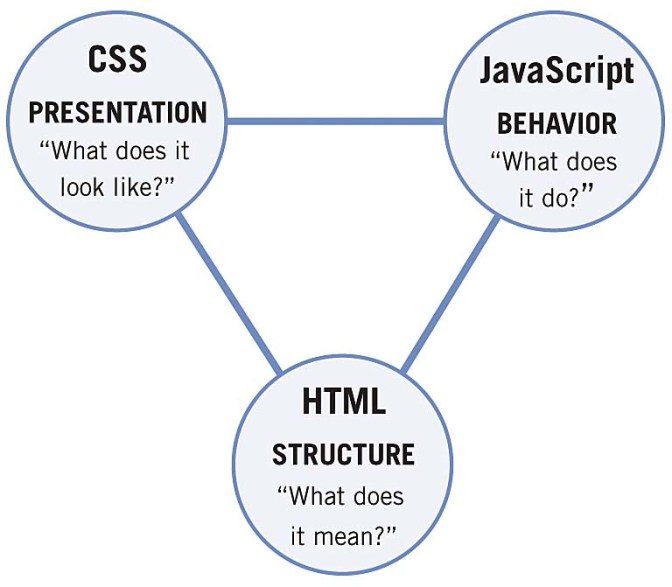
\includegraphics[width=\textwidth]{html-css-js}
https://melaloo.wordpress.com/2015/07/12/intiwebsites-for-dummies-what-are-html-css-javascript-and-php/

Przeglądarka internetowa pobiera strony internetowe używając protokołu HTTP.
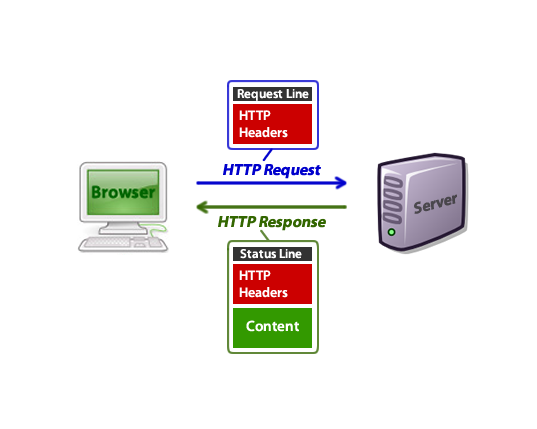
\includegraphics[width=\textwidth]{http_diagram}
https://code.tutsplus.com/tutorials/http-headers-for-dummies--net-8039


%%% TODO DIAGRAMY SEKWENCJI (UML!!)
\subsection{Wstęp do architektury systemu - widok z lotu ptaka}
Na architekturę produktu składa się:
\begin{itemize}
    \item Aplikacja przeglądarkowa (front-end)
    \item Aplikacja strony serwerowej (back-end)
    \item Baza danych
\end{itemize}
Front-end jest aplikacją wykonującą się na urządzeniu użytkownika. Zapytania o dane i wysyłanie danych do aplikacji strony serwerowej za pomocą HTTP Api. Strona serwerowa komunikuje się z bazą danych za pomocą JDBC.
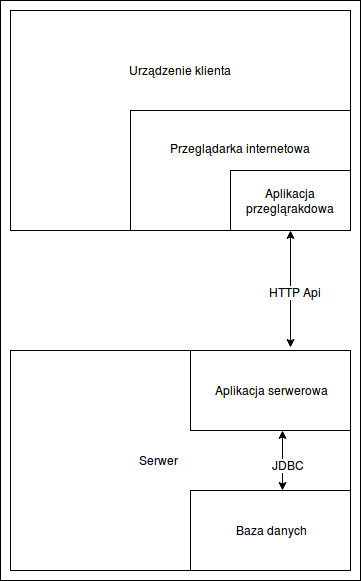
\includegraphics{komunikacja-serwer-klient-okolny}



\subsubsection{Architektura aplicaji serwerowej}
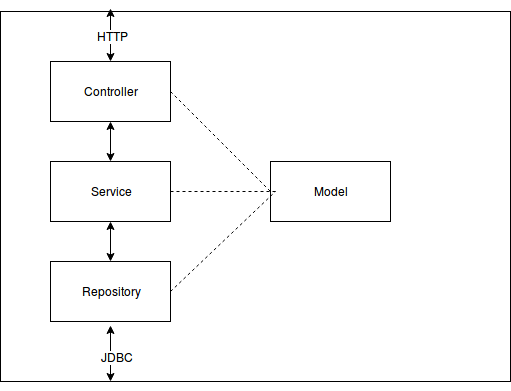
\includegraphics[width=\textwidth]{backedn-schema}
\begin{itemize}
    \item Controller - warstwa odpowiedzialna za odbieranie zapytań HTTP i przetwarzanie ich na obiekty JVM-owe oraz za przetwarzanie odpowiedzi (obiektów JVM-owych) na waidomości HTTP i odsyłanie ich.
    \item Service - warstwa pośrednicząca międzu Controller-em a Repository-em. Przetwarza zapytania otrzymane od Controllera na zapytania dla Repository i przetwarza odpowiedzi od Repository na odpowiedzi dla Controller-a.
    \item Repository - warstwa odpowiedzialna za wykonywanie zapytań do bazy danych.
    \item Model - wspóny dla wyżej wymienionych warstw sposób reprezentacji encji jako obiektów JVM-kowych, który może być przetworzony na JSON-a (na potrzeby HTTP API) lub repotezentację bazodanową (na potrzeby bazy danych). Umożliwia komunikację pomiędzy Controller-em, Servic-em i Repository-em.
\end{itemize}

\subsubsection{Architektuwa aplikacji przeglądarkowej}
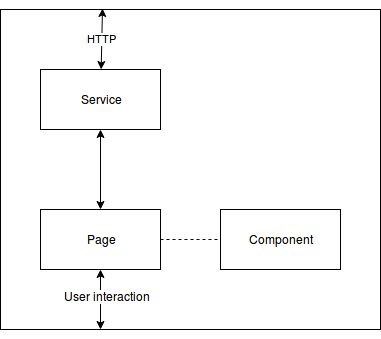
\includegraphics[width=\textwidth]{front-schema}
\begin{itemize}
    \item Service - serwisy odpowiadają za wysyłanie zapytań do aplikacji serwerowej i odbieranie odpowiedzi
    \item Page - Trasowalna strona wyświatlana użytkownikowi
    \item Component - Strony korzystają z komponentów
\end{itemize}

\subsubsection{Komunikcja aplikacji serwerowej i klienckiej}
\emph{TODO przekleić wszystko ze Słagera xDDDD}


\subsection{Baza danych}
Schemat relacyjnej bazy danych:
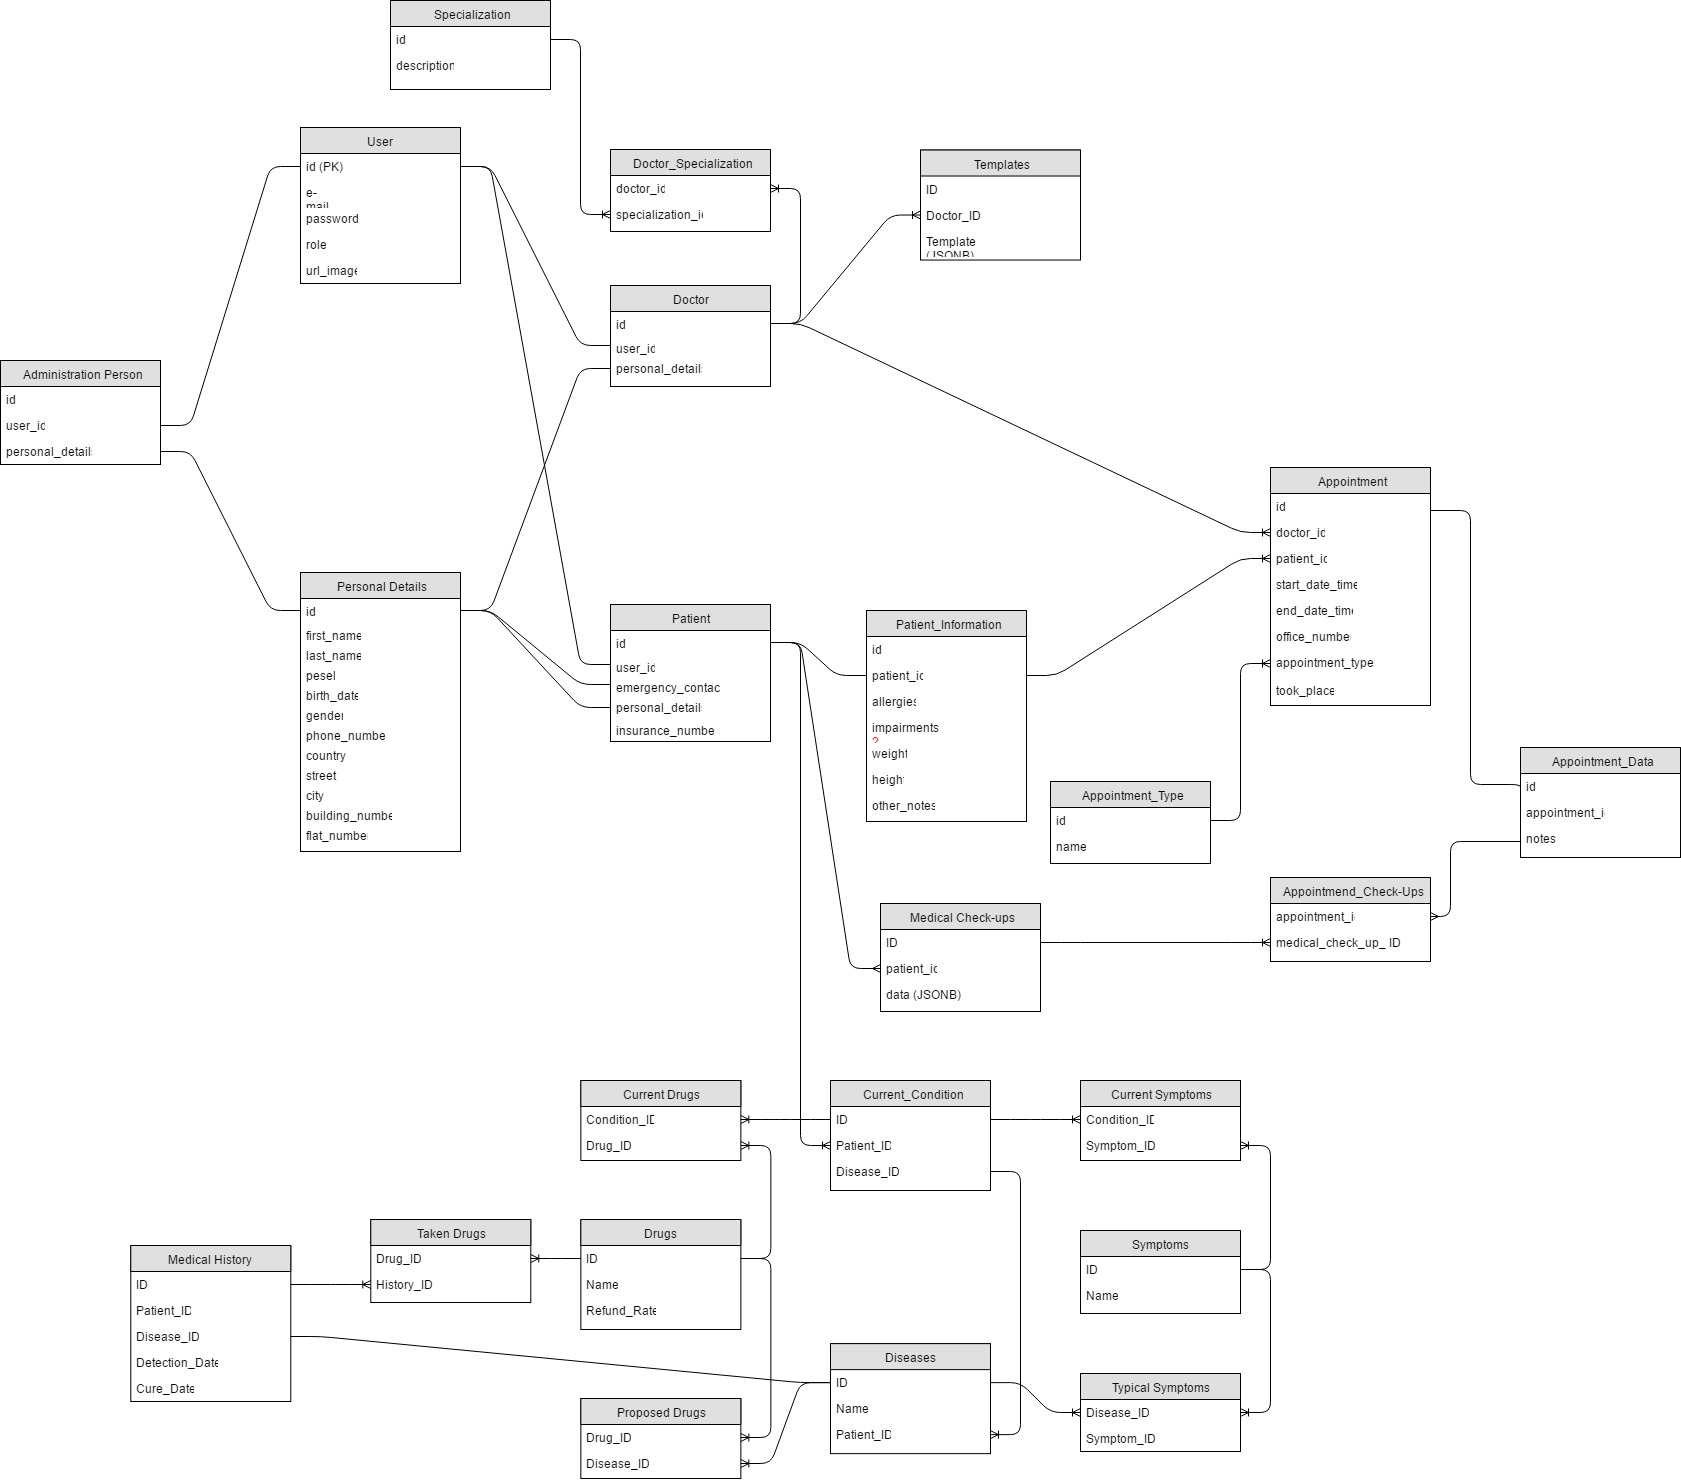
\includegraphics[width=\textwidth]{db-schema}

\subsection{Aplikacja strony serwerowej}
\subsubsection{Modelowane encje}
    \paragraph{Timeslot} - możliwy termin wizyty u danego lekarza.\\
    Nie zawiera informacji czy termin jest zarezerwowany, może być interpretowany jako czas w którym lekarz na pewno jest w pracy \\
    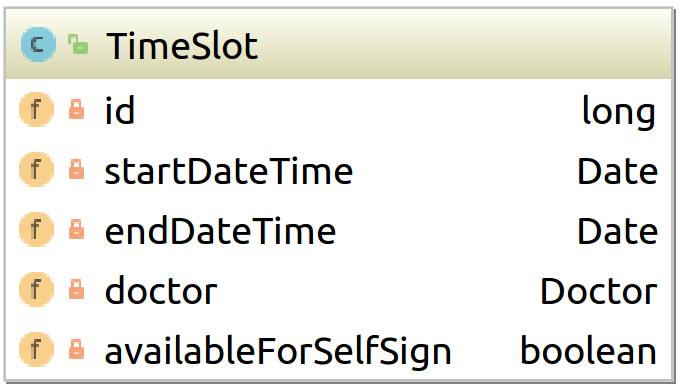
\includegraphics[width=\textwidth]{TimeSlot}
    \paragraph{Appointment} - Zarezerwowany termin u wizyty \\
    Zawiera szczegóły rezerwacji, jak na przykład dane pacjenta czy priorytet wizyty.
    Zawieta w sobie \emph{TimeSlot} - czyli informację o terminie i lekarzu przyjmującym wizytę \\
    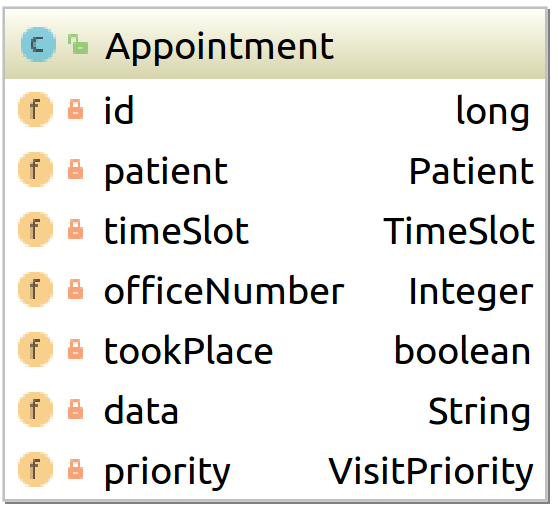
\includegraphics[width=\textwidth]{Appointment}
    \paragraph{Doctor} - lekarz \\
    Encja lekarza odpowiada jednej jego specjalizacji \\
    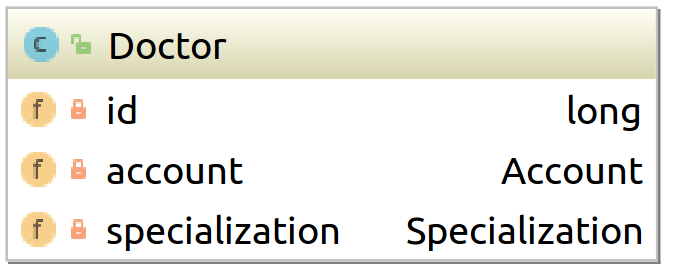
\includegraphics[width=\textwidth]{Doctor}
    \paragraph{Patient} - pacjent \\
    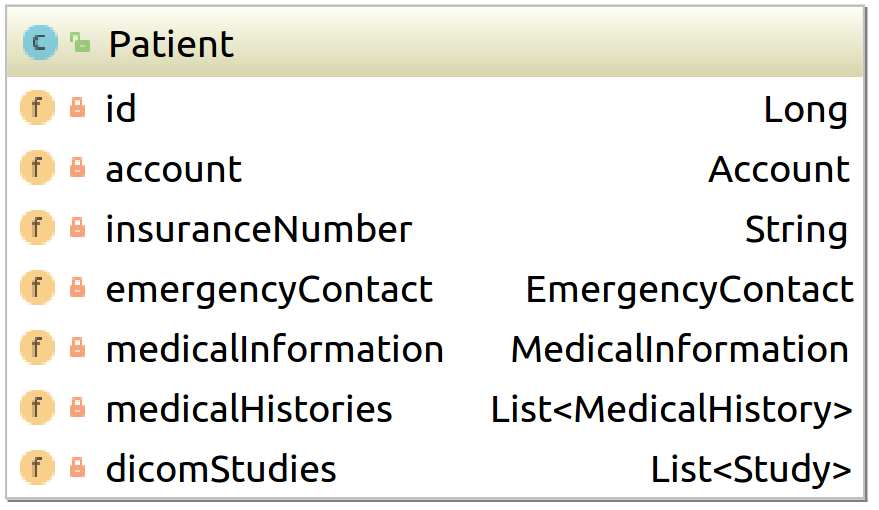
\includegraphics[width=\textwidth]{Patient}
    \paragraph{Account} - konto w systemie \\
    Konto nie opisuje uprawnień ani hasła użytkownika, jest tylko łącznikiem dla endji \\
    Account zawiera \emph{User} które ma hasło i e-mail użytkownika.
    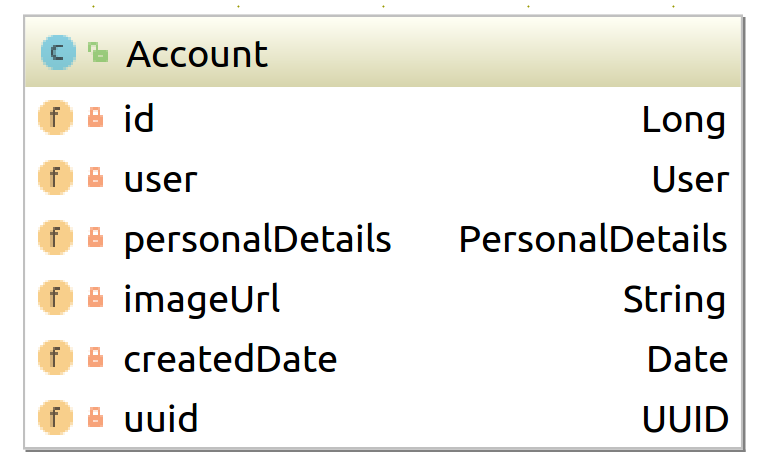
\includegraphics[width=\textwidth]{Account}
    \paragraph{PersonalDetails} - dane osobowe \\
    Ta encja dotyczy zarówno lekarza i pacjenta \\
    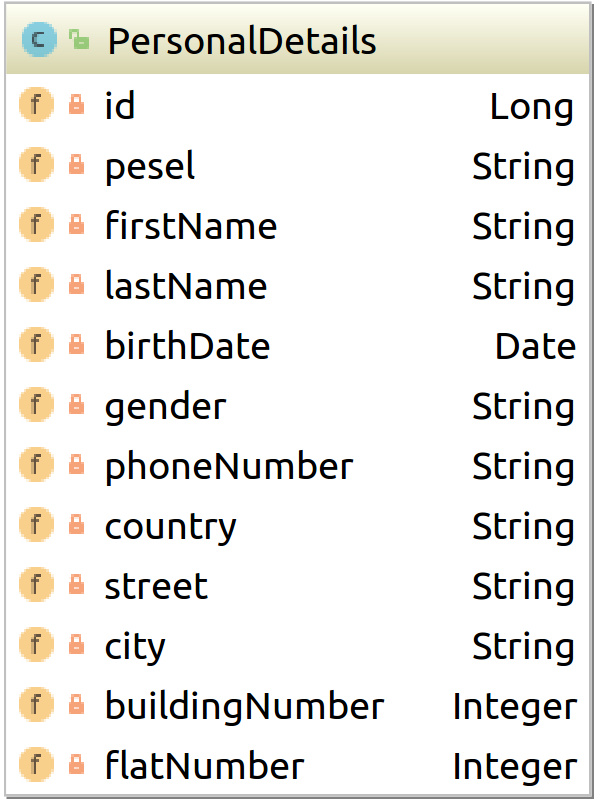
\includegraphics[width=\textwidth]{PersonalDetails}
    \paragraph{User} - dane użytkownika \\
    powiązane z \emph{Account} \\
    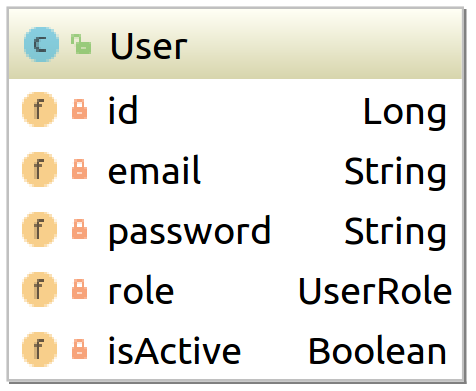
\includegraphics[width=\textwidth]{User}
    \paragraph{Specialization} - specjalizacja lekarza \\
    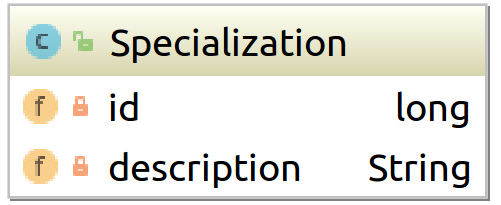
\includegraphics[width=\textwidth]{Specialization}
\subsubsection{Powiązanie modelowanych encji}
\paragraph{Wersja zwinięta} - Schemat bez widocznych pól\\
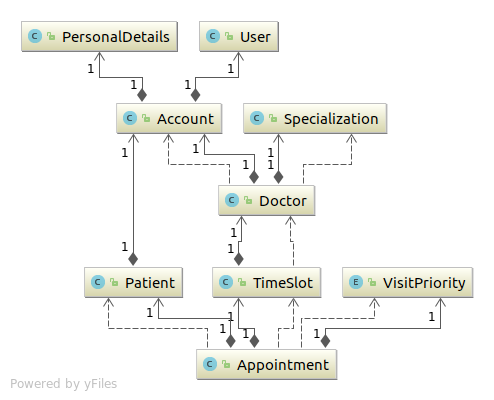
\includegraphics[width=\textwidth]{java-entities-small}
\paragraph{Wersja rozwinięta} - Schemat z widocznymi polami \\
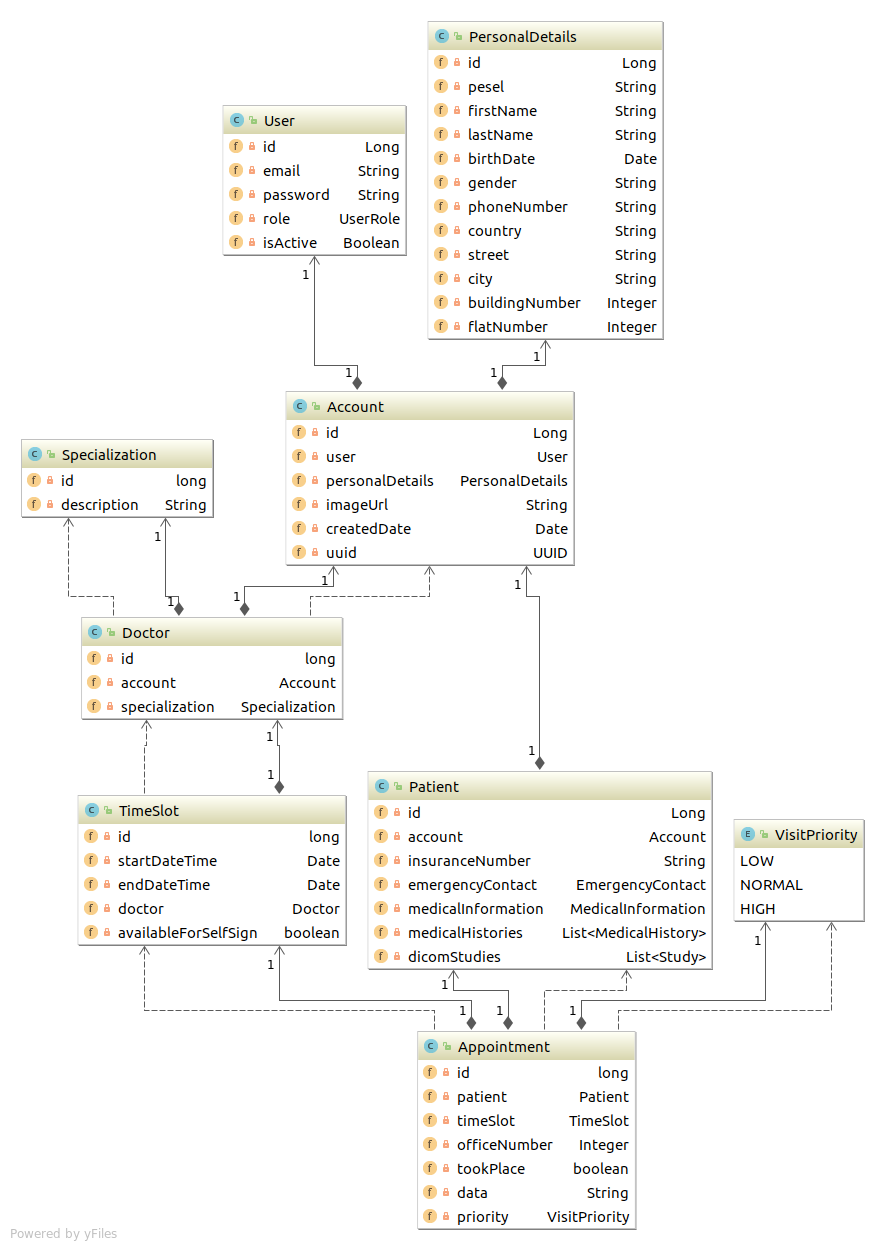
\includegraphics[width=\textwidth]{java-entities-big}

\section{Organizacja pracy}
%\section{Work organization}
\label{sec:organizacja-pracy}

\emph{Struktura zespołu (role poszczególnych osób), krótki opis i
  uzasadnienie przyjętej metodyki i/lub kolejności prac, planowane i
  zrealizowane etapy prac ze wskazaniem udziału poszczególnych
  członków zespołu, wykorzystane praktyki i narzędzia w zarządzaniu
  projektem.}
  
\subsection{Strunktura zespołu}
\subsubsection{Hierarchia zarządzania}
W zepole wyróżniony jest przywódca. Wyróżnianie innych funkcji wydało nam się zbędne.
\begin{itemize}
    \item Wojciech Karpiel - szef, odpowiedzialny za komunikację z Klientem i współpracującymi zespołami
    \item Fiip Galas - członek zespołu
    \item Michał Hamuda - członek zespołu
\end{itemize}
\subsubsection{Podział technologiczny}
Rozważaliśmy wprowadzenie podziału ze względu na kompetencje techniczne, czyli:
\begin{itemize}
    \item Osoba zajmująca się stroną serwerową
    \item Osoba zajmująca się aplikacją przeglądarkową
\end{itemize}
Uznaliśmy to za zabyteczne ponieważ produkt składa się głównie z kodu front-endowego i taki podział funkcji spowodowałby nierównomierny podział prac. Zamiast tego każdy członek zespołu odpowiadał za stworzenie front-endowej i back-endowej części funkcjonalności którą wdrażał.

\subsection{Wyznaczanie zadań i podział prac}
Wykorzystywaliśmy Jira-ę, hostowaną przez IISG. Po każdym spotkaniu z Klientem szef zespołu przetwarzał wymagane przez Klienta funkcjonalności na Jira-owe bilety. Każdy bilet opisywał jedną funkcjonalność. Bilety były posortowane wegług ważności (to znaczy: funckjonalności które należało zaimplementować do następnego spotkania z klientem były najwyżej, najniżej były nasze pomysły których Klient nie wymagał). Członkowie zespołu, według czasu i możliwości, przypisywali sobie zadania i wykonywali je.

\subsection{Sposób wykonywania zadań}
Produkt składa się de facto z dwóch powiązanych pod-projektów: części front-endowej i back-enbdowej. Te dwa pod-projekty były objęte systemem kontroli wersji Git. Dla każdego pod-projektu osobno członek zespołu tworzył Git-ową gałąź przypisaną funkcjonalności i na niej komitował kod wprowadzający funkcjowalność. Po zakończeniu pracy, pozostali członkowie zespołu przeglądali kod na gałęzi i ewentualnie prosili o wprowadzenie poprawek (code-review). Na końcu gałąź funkcjonalnościowa była dołączana do głównej gałęzi.

\subsection{Komunikacja z powiązanymi zespołami}
\subsubsection{Komunikacja bieżąca}
Do komunikacji bieżącej używaliśmy komunikatora Skype. Według potrzeb, umawialiśmy się na ta zwane call-e, podczas których przedstawiciele każdego z powiązanych zespołów omawiali stan prac i planowali przyszłą pracę.
\subsubsection{Wymiana wiedzy}
Używaliśmy Confluence-a, hostowanego przez IISG. Służył on jako pamięć długotrwała oraz punkt wymiany informacji między zespołami. Tam spisywaliśmy notatki ze spotkań (zarówno tych z Klientem jak i między-zespołowych), prowadziliśmy kalendarz przyszłych spotkań oraz spisywaliśmy różnorakie informacje które wydawały się nam przydatne. Do tego Confluence-a mieli dostęp również członkowie powiązanych zespołów.

\subsection{Spotkania z Klientem}
Naszym Klientem był dr Bartłomiej Śnieżyński, natomiast Klientem powiązanych zespołów był dr Piotr Nawrocki. Razem z zespołami powiązanymi prosiliśmy naszych Klientów o wspólne spotkania (3 zespoły i 2 Klientów), na co nasi Klienci chętnie przystali. Taka organizacja spotkań ułatwiła koordynację i integrację zespołów.
  
  %% Koniec organizacji pracy!



\section{Wyniki projektu}
%\section{Project results}

\label{sec:wyniki-projektu}

\emph{Wskazanie wyników projektu (co konkretnie udało się uzyskało:
  oprogramowanie, dokumentacja, raporty z testów/wdrożenia, itd.), prezentacja wyników
  i ocena ich użyteczności (jak zostało to zweryfikowane --- np.\ wnioski
  klienta/użytkownika, zrealizowane testy wydajnościowe, itd.),
  istniejce ograniczenia i propozycje dalszych prac.}

\subsection{Wymagania dla uruchomiania aplikacji}
\subsubsection{Wymagania techniczne dla klienta}
\begin{itemize}
  \item  Połączenie z serwerem Health-Menagera (zazwyczaj realizowane przez sieć Internet)
  \item Przeglądarka internetowa zdolna do obsługi ECMAScript-u w wersji 6 lub późniejszej (na przykład Mozilla Firefox w wersji 56.0)
\end{itemize}

\subsubsection{Wymagania techniczne dla serwera}
\begin{itemize}
    \item Połączenie z siecią komuterową w której znajdują się użytkownicy
    \item Java Runtime Environment w wersi 8 lub późniejszej (na przykład \href{https://www.java.com/pl/download/manual.jsp}{JRE firmy Oracle}
    \item Baza danych PostgreSQL
    \item Serwer HTTP (TODO)
\end{itemize}

\subsubsection{Wymagania techniczne dla programisty}
\begin{itemize}
    \item \href{https://www.npmjs.com/}{NPM - Next Popular Module}
    \item Java Developement Kit w wersi 8 lub późniejszej
    \item Gradle
    \item Baza danych Postgresql
\end{itemize}


\subsection{Konfiguracja aplikacji}
\subsubsection{Aplikacja przeglądarkowa}{Należy ustawić:
\begin{itemize}
    \item port na którym będzie wystawione GUI (przez HTTP)
    \item Adres end-pointu back-endowego
\end{itemize}}
\subsubsection{Aplikacja serwerowa}{Należy ustawić:
\begin{itemize}
    \item Parametry połączenia z bazą danych
\end{itemize}}
\paragraph{Baza danych}{Prawidłowo skonfigurowana aplikacja serwerowa powinna utworzyć schemat bazy danych w przypadku jego nieistnienia}


\subsection{Przewodnik użytkownika}
\subsubsection{Administrator}
\paragraph{Rejestracja użytkownika}{}
\paragraph{Utrzymanie aplikacji}{}
\subsubsection{Lekarz}
\paragraph{Ustalanie grafiku}{}
\paragraph{Drukowanie grafiku}{}
\paragraph{Ustalanie terminów}{}
\paragraph{Rejestracja pacjenta}{}
\paragraph{Eksport kalendarza}{}
\subsubsection{Pacjent}
\paragraph{Rejestracja}{}
\paragraph{Logowanie}{}
\paragraph{Zapis na wizytę}{}
\paragraph{Eksport kalendarza}{}
\subsubsection{Recepcjonistka}
\paragraph{Rejestracja pacjenta}{}
\paragraph{Zmiana terminu wizyty}{}

%%%%% KONIEC %%%%%%
% o ile to mozliwe prosze uzywac odwolan \cite w konkretnych miejscach a nie \nocite

\nocite{artykul2011,ksiazka2011,narzedzie2011,projekt2011}

\bibliography{bibliografia}

\end{document}
